\scanpage{13}
Comme $\operatorname{int}(l_0)\sigma_\infty$ fixe\textsuperscript{\unsure{6|$\sigma$}} $l_\infty$ (mais n'est peut-être pas de carré $l_\infty$), on doit le multiplier à droite par un $\operatorname{int}(l_\infty^\alpha)$
\figure{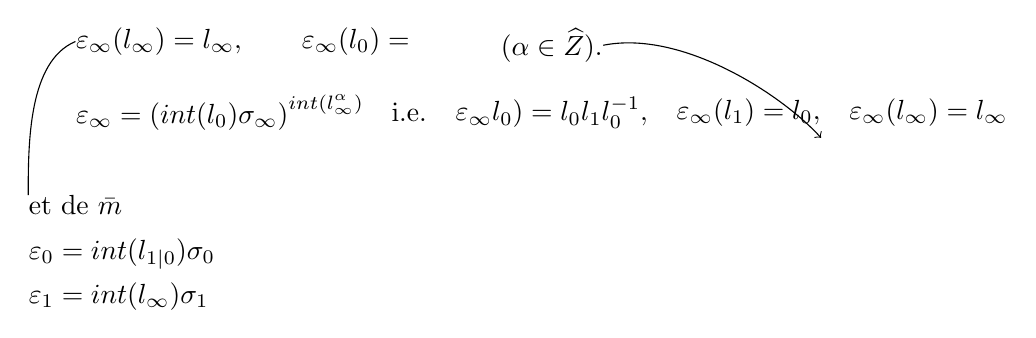
\begin{tikzpicture}[x=1cm,y=1cm]
\node[anchor=west,inner sep=0pt] (def) at (0,0) {$\varepsilon_\infty=(\operatorname{int}(l_0)\sigma_\infty)\raisebox{1.2ex}{$\scriptstyle\inserted{\operatorname{int}(l_\infty^\alpha)}$}$};
\node[anchor=west,xshift=10pt,inner sep=0pt] (ie) at (def.east) {i.e.};
\node[anchor=west,xshift=10pt,inner sep=0pt] (a0) at (ie.east) {$\varepsilon_\infty l_0)=l_0l_1l_0^{-1},$};
\node[anchor=west,xshift=10pt,inner sep=0pt] (a1) at (a0.east) {$\varepsilon_\infty(l_1)=l_0,$};
\node[anchor=west,xshift=10pt,inner sep=0pt] (ai) at (a1.east) {$\varepsilon_\infty(l_\infty)=l_\infty$};
\node[anchor=west,inner sep=0pt] (cancel) at (0,.9) {$\deleted{\varepsilon_\infty(l_\infty)=l_\infty,\qquad\varepsilon_\infty(l_0)=}$};
\node[anchor=south,yshift=12pt,inner sep=0pt] (cond) at (a0.north) {$(\alpha\in\widehat{\mathbb Z})$.};
\draw[->] (cond.east) .. controls +(1.0,.2) and +(-.5,.55) .. ([yshift=-4pt]a1.south east);
\node[anchor=north west,align=left,inner sep=0pt] (other) at (-.6,-1.05) {\deleted{et de $\bar m$}\\[4pt]
$\deleted{\varepsilon_0=\operatorname{int}(l_{\unsure{1|0}})\sigma_0}$\\[4pt]
$\deleted{\varepsilon_1=\operatorname{int}(l_\infty)\sigma_1}$};
\draw (cancel.west) .. controls +(-.6,-.25) and +(0,.65) .. (other.north west);
\end{tikzpicture}}
On \deleted{aura \unsure{donc}} \inserted{doit écrire $\varepsilon_{\unsure{\infty|0}}^2=l_\infty$..} Ecrivant $g$ au lieu de $\operatorname{int}(g)$ pour $g\in\unsure{\pi|\Pi}$, i.e. identifiant $\unsure{\pi|\Pi}$ à un ss-groupe de $\operatorname{Aut}(\unsure{\pi|\Pi})$, je \deleted{\unsure{trouve}} \inserted{\unsure{écris}}
\deleted{\unsure{comme} $\varepsilon_\infty=l_0\sigma_\infty$}.
\[
\varepsilon_\infty=l_0\sigma_\infty l_\infty^\alpha.
\]
\deleted{\[
\varepsilon_\infty^2=l_0\sigma_\infty l_0\sigma_\infty
=l_0\sigma_\infty l_0\sigma_\infty^{-1}=l_0\sigma_\infty(l_0)
\]}
donc
\[
\begin{aligned}
\varepsilon_\infty^2&=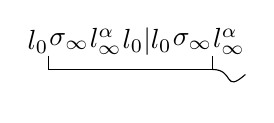
\begin{tikzpicture}[baseline=(a.base)]
\node[inner sep=0pt] (a) at (0,0) {$l_0$};
\node[anchor=west,inner sep=0pt] (b) at (a.east) {$\sigma_\infty$};
\node[anchor=west,inner sep=0pt] (c) at (b.east) {$l_\infty^\alpha$};
\node[anchor=west,inner sep=0pt] (d) at (c.east) {$\unsure{l_0|\deleted{l_0}}$};
\node[anchor=west,inner sep=0pt] (e) at (d.east) {$\sigma_\infty$};
\node[anchor=west,inner sep=0pt] (f) at (e.east) {$l_\infty^\alpha$};
\draw ([yshift=-2pt]b.south west)--([yshift=-7pt]b.south west)--([yshift=-7pt]e.south east)--([yshift=-2pt]e.south east);
\draw ([yshift=-7pt]e.south east) .. controls +(8pt,0) and +(-8pt,-7pt) .. ([yshift=-7pt]f.south east);
\end{tikzpicture}\\
&=l_0\sigma_\infty(l_\infty^\alpha l_0)l_\infty^\alpha
=l_0(l_0^{-1}l_1^{-1})^\alpha l_1(l_1^{-1}l_0^{-1})^\alpha\\
&=\underbrace{\deleted{l_0\sigma_\infty(l_\infty)}}_{\inserted{l_0l_\infty.}}\deleted{\sigma_\infty(l_\infty)^{\alpha-1}\sigma_\infty(l_0)l_\infty^\alpha}
\end{aligned}
\]
et la relation $\varepsilon_\infty^2=l_\infty$ \inserted{\deleted{$\unsure{(=)|(\Rightarrow)}l_1^{-1}l_{\unsure{0|\infty}}^{-1}$}} s'écrit aussi, en multipliant par $l_0l_1$
\deleted{\[
l_0l_\infty\underbrace{\sigma_\infty(l_\infty)^{\alpha-1}}_{(l_0^{-1}l_1^{-1})^{\alpha-1}}\underbrace{\sigma_\infty(l_0)}_{l_1}l_\infty^{\alpha-1}=1
\]}
i.e.
\deleted{\[
\deleted{\unsure{l_\infty^{-1}l_1|l_\infty^{-1}l_\infty|l_0^{-1}l_1}}l_0^{1-\alpha}l_1^{2-\alpha}l_\infty^\alpha=1
\]}
\[
l_0l_1l_0(l_0^{-1}l_1^{-1})^\alpha l_1(l_1^{-1}l_{\unsure{0|\infty}}^{-1})^\alpha=1
\]
\margin{\unsure{prends|prenons|pour} $\alpha\unsure{=|\ge}\unsure{2|1}$ ?}
\deleted{\[
l_0l_1l_0l_0^{-1}l_1^{-1}l_0^{-1}l_1^{-1}l_1l_1^{-1}l_0^{-1}l_1^{-1}l_0^{-1}=1?\qquad\text{Non !}
\]}
\[
\deleted{l_0}\deleted{l_1}\deleted{l_0}\deleted{l_0^{-1}}\deleted{l_1^{-1}}\deleted{l_1}\deleted{l_1^{-1}}\deleted{l_0^{-1}}=1
\qquad\text{OK}\qquad\text{donc}
\]
\[
\left\{\begin{aligned}
\varepsilon_\infty&=l_0\sigma_\infty l_\infty\quad\text{(ou encore }\operatorname{int}(l_0)\sigma_\infty\operatorname{int}(l_\infty)\text{)}\\
\varepsilon_0&=l_1\sigma_0l_0\\
\varepsilon_1&=l_\infty\sigma_1l_1
\end{aligned}\right.
\]
\mspage{12}
